\chapter{リポジトリ — プロジェクトの器を作る}

\section{この章で学ぶこと}

ソフトウェア開発において、プロジェクトのファイルを管理するための「入れ物」が必要です。Gitではこの入れ物を\textbf{リポジトリ（repository）}と呼びます。略して「リポ」や「repo」と呼ばれることもあります。リポジトリは単なるフォルダではなく、ファイルの現在の状態だけでなく、過去のすべての変更履歴を保持する特別な構造を持っています。

この章では、以下のことを学びます。

\begin{itemize}
  \item リポジトリの内部構造と \cmd{.git} フォルダの役割
  \item リポジトリを作成する3つの方法と、それぞれの適切な使い分け
  \item \cmd{git clone} コマンドの詳細な動作とオプション
  \item リモートリポジトリ（remote）の概念と管理方法
  \item \cmd{.gitignore} によるファイル除外の仕組みと実践的な書き方
  \item GitHub上でのリポジトリ設定（可視性、ブランチ保護、テンプレート）
\end{itemize}

リポジトリの作成はGitを使ったすべての作業の出発点です。この章の内容をしっかり理解することで、以降の章で扱うブランチ操作やコミットの意味がより深く理解できるようになります。

\section{リポジトリの構造 — .gitフォルダの役割}

\subsection{プロジェクトフォルダとリポジトリの関係}

まず、「リポジトリ」と「普通のフォルダ」の違いを理解しましょう。たとえば、あなたが \cmd{my-project} というフォルダを作り、その中にソースコードやドキュメントを置いたとします。この段階では、それはただのフォルダです。ここで \cmd{git init} コマンドを実行すると、フォルダの中に \cmd{.git} という隠しディレクトリが作成されます。この \cmd{.git} ディレクトリが存在することで、普通のフォルダが「リポジトリ」に変わるのです。

\begin{figure}[htbp]
\centering
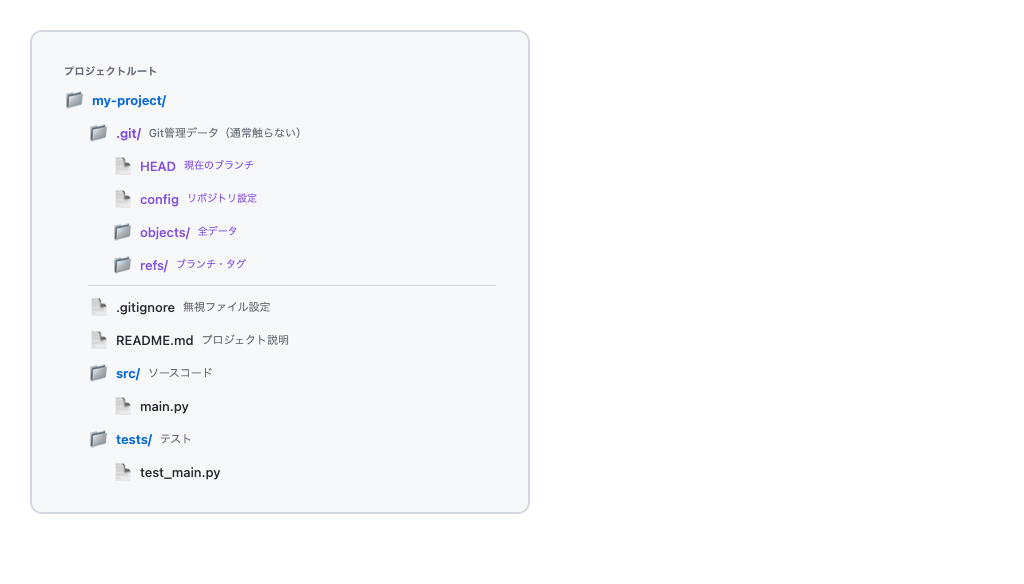
\includegraphics[width=0.9\textwidth]{images/diagram-repo-structure.png}
\end{figure}

\subsection{.gitフォルダの中身}

\cmd{.git} フォルダは「リポジトリの心臓部」とも言える存在です。この中には、プロジェクトの過去から現在に至るまでのすべての変更履歴が格納されています。通常、この中のファイルを手動で操作する必要はありませんが、その構造を理解しておくと、Gitの動作原理がより明確になります。

\textbf{HEAD} ファイルには、現在作業しているブランチの情報が書かれています。たとえば \cmd{ref: refs/heads/main} という内容であれば、今 \cmd{main} ブランチにいることを意味します。

\textbf{objects/} ディレクトリは、Gitのデータベースそのものです。ファイルの内容（blob）、ディレクトリ構造（tree）、コミット情報（commit）がすべてハッシュ値で管理され、この中に保存されています。Gitが「分散型バージョン管理」と呼ばれるのは、この \cmd{objects/} ディレクトリにリポジトリの完全な履歴が含まれているからです。GitHubのサーバーがダウンしても、あなたのローカルに完全な履歴が残っています。

\textbf{refs/} ディレクトリには、ブランチやタグの「ポインタ」が保存されています。ブランチとは、特定のコミットを指し示す軽量なポインタに過ぎないのです（これについては第7章で詳しく解説します）。

\textbf{config} ファイルには、このリポジトリに固有の設定が保存されます。リモートリポジトリのURLや、ブランチの追跡情報などがここに記録されます。

\begin{quote}
\textbf{重要}: \cmd{.git} フォルダを削除すると、すべての変更履歴が失われます。プロジェクトのファイル自体は残りますが、Gitの管理下ではなくなります。\cmd{.git} フォルダには絶対に触れないようにしましょう。
\end{quote}

\section{リポジトリの作成方法}

リポジトリを作成する方法は大きく分けて3つあります。それぞれの方法には適した場面がありますので、状況に応じて使い分けましょう。

\subsection{方法1: GitHubで作成してからクローン（推奨）}

最も一般的で、初心者にも推奨される方法です。この方法では、まずGitHubのWebインターフェース上でリポジトリを作成し、それをローカルにコピー（クローン）します。

なぜこの方法が推奨されるのでしょうか。それは、GitHubで作成する際にREADMEファイルや \cmd{.gitignore}、ライセンスファイルなどの初期ファイルを自動生成できるからです。また、リモートリポジトリとの接続設定が自動的に行われるため、設定ミスが起きにくいという利点もあります。

\textbf{GitHub上での操作手順:}

\begin{enumerate}
  \item GitHubにログインし、画面右上の「\textbf{+}」ボタンをクリックします
  \item ドロップダウンメニューから「\textbf{New repository}」を選択します
\end{enumerate}

\begin{figure}[htbp]
\centering
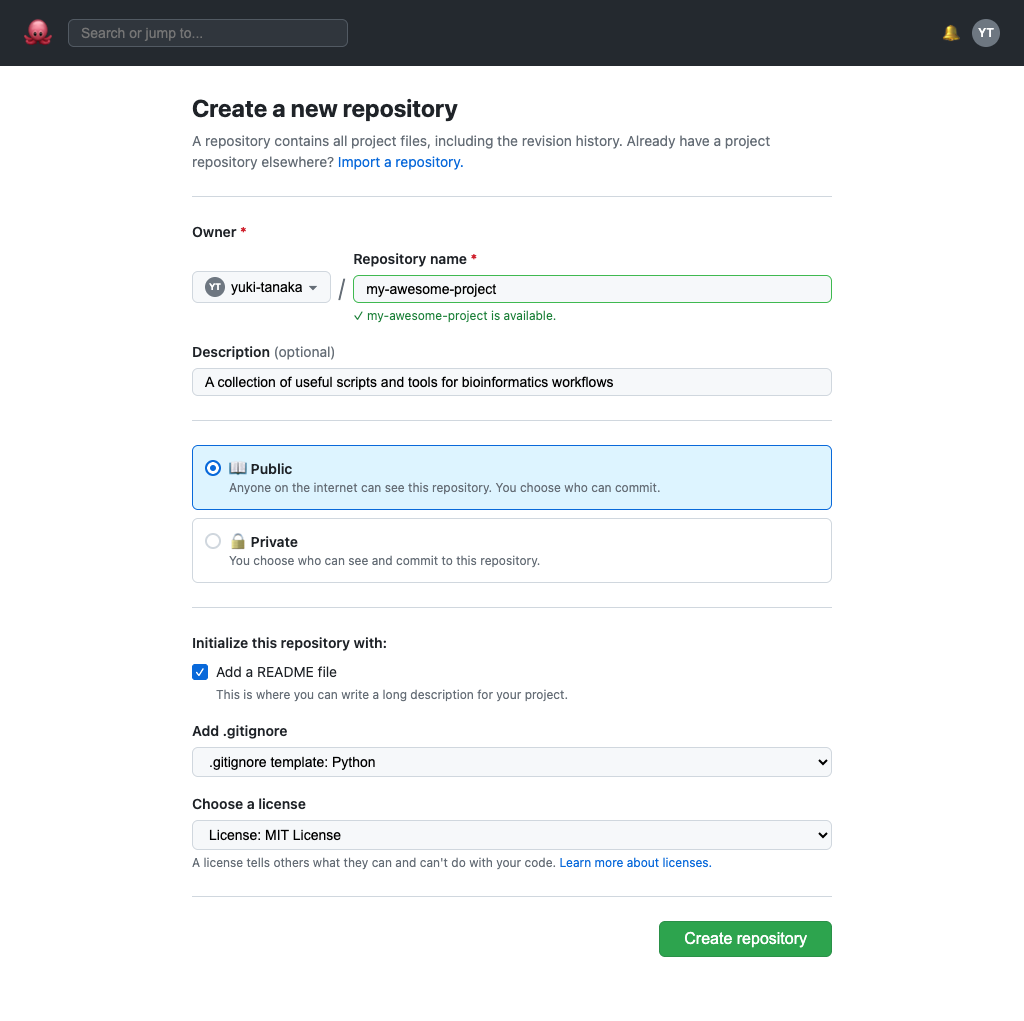
\includegraphics[width=0.95\textwidth]{images/repo-create.png}
\caption{GitHub右上の+ボタンとドロップダウンメニュー}
\end{figure}

3. リポジトリの作成画面で、以下の項目を設定します

\begin{table}[htbp]
\centering
\begin{tabular}{llp{6cm}}
\hline
\textbf{項目} & \textbf{説明} & \textbf{推奨設定} \\
\hline
\textbf{Repository name} & リポジトリ名。URLの一部になる & プロジェクト内容がわかる簡潔な名前 \\
\textbf{Description} & リポジトリの簡単な説明文（任意） & 1行で内容がわかる説明を書く \\
\textbf{Public / Private} & 公開・非公開の選択 & 学習目的ならPublicでOK \\
\textbf{Add a README file} & README.mdを自動生成するか & チェック推奨 \\
\textbf{Add .gitignore} & 言語に応じた.gitignoreテンプレートを選択 & 使用する言語を選択 \\
\textbf{Choose a license} & オープンソースライセンスの選択 & OSSの場合はMITなどを選択 \\
\hline
\end{tabular}
\end{table}

\begin{figure}[htbp]
\centering
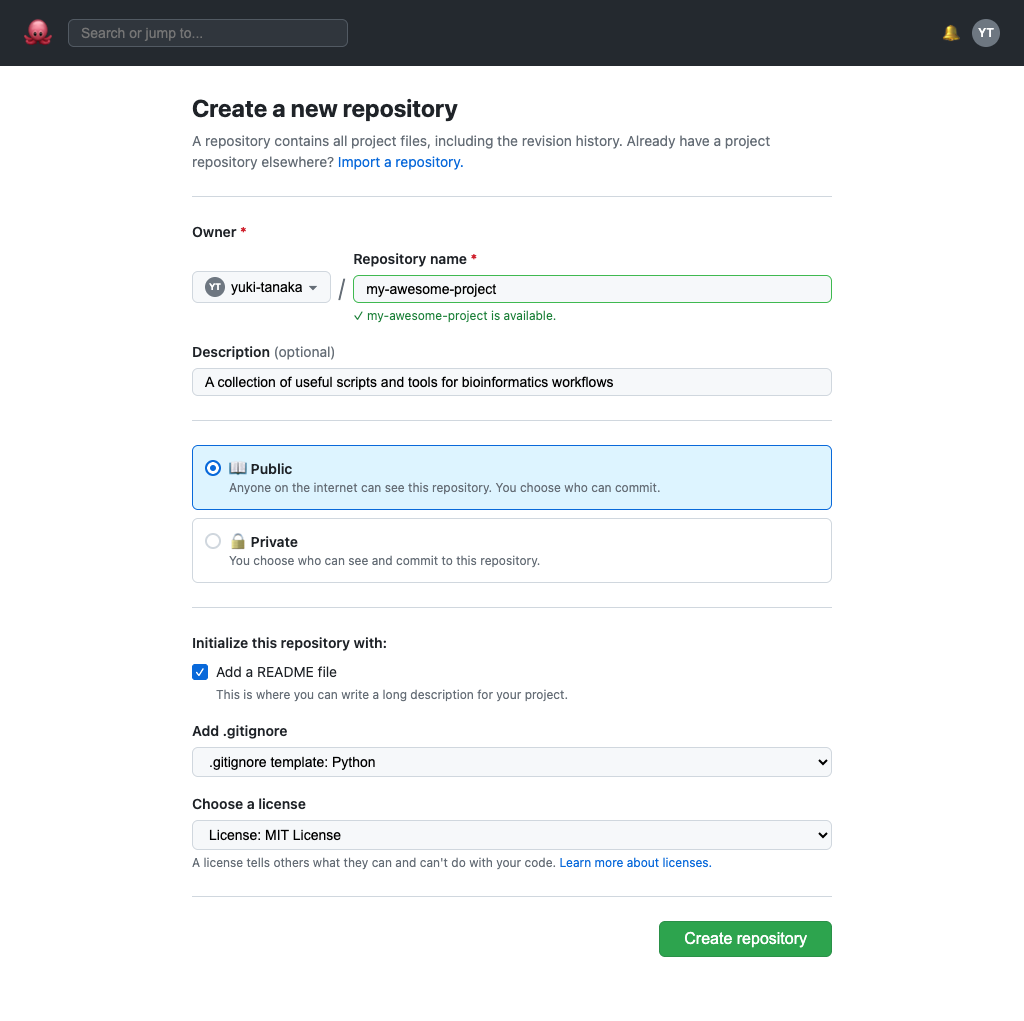
\includegraphics[width=0.95\textwidth]{images/repo-create.png}
\caption{リポジトリ作成画面の各項目}
\end{figure}

4. 「\textbf{Create repository}」ボタンをクリックして作成完了です

\textbf{ローカルにクローンする:}

GitHubでリポジトリが作成できたら、次はそれをローカルのPCにコピーします。リポジトリのページにある「\textbf{Code}」ボタンをクリックすると、クローン用のURLが表示されます。

\begin{figure}[htbp]
\centering
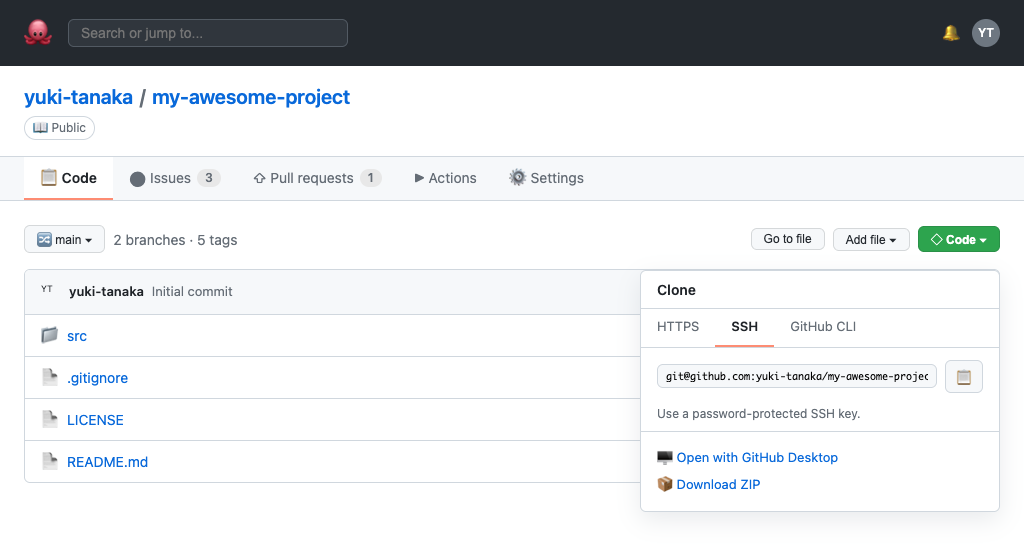
\includegraphics[width=0.95\textwidth]{images/clone-url.png}
\caption{Codeボタンをクリックした状態のクローンURL表示}
\end{figure}

\begin{lstlisting}[language=bash]
# SSH接続を使う場合（第4章で設定済みなら推奨）
git clone git@github.com:username/my-project.git

# HTTPS接続を使う場合
git clone https://github.com/username/my-project.git

# GitHub CLIを使う場合（最もシンプル）
gh repo clone username/my-project
\end{lstlisting}

クローンが完了したら、作成されたディレクトリに移動して作業を始めます。

\begin{lstlisting}[language=bash]
cd my-project
\end{lstlisting}

\subsection{方法2: ローカルで作成してからGitHubにプッシュ}

既にローカルで開発を始めているプロジェクトをGitHub管理に移行したい場合や、ローカルでの初期作業を先に行いたい場合は、この方法を使います。

この方法では、まずローカルでGitリポジトリを初期化し、最初のコミットを作成した後、GitHubにリモートリポジトリを作成して接続します。各コマンドの意味を順に見ていきましょう。

\begin{lstlisting}[language=bash]
# ステップ1: プロジェクトフォルダを作成して移動する
mkdir my-project
cd my-project

# ステップ2: Gitリポジトリとして初期化する
# このコマンドで .git フォルダが作成される
git init

# ステップ3: READMEファイルを作成する
echo "# My Project" > README.md

# ステップ4: ファイルをステージングしてコミットする
git add README.md
git commit -m "Initial commit"
\end{lstlisting}

\cmd{git init} は、カレントディレクトリに \cmd{.git} フォルダを作成し、そのフォルダをGitリポジトリとして初期化するコマンドです。この時点ではまだGitHubとの接続はありません。完全にローカルだけのリポジトリです。

次に、GitHubにリモートリポジトリを作成して接続します。GitHub CLIがインストールされている場合は、1つのコマンドで完了します。

\begin{lstlisting}[language=bash]
# GitHub CLIを使う場合（リモート作成・接続・プッシュを一括実行）
gh repo create my-project --public --source=. --remote=origin --push
\end{lstlisting}

このコマンドのオプションの意味は次のとおりです。\cmd{--public} はリポジトリをPublic（公開）として作成することを指定します。\cmd{--source=.} はカレントディレクトリをソースとして使うことを意味します。\cmd{--remote=origin} はリモート接続名を \cmd{origin} に設定します。\cmd{--push} はローカルのコミットを即座にプッシュします。

\textbf{GitHub CLIを使わない場合}は、まずGitHubのWebインターフェースで空のリポジトリを作成します（このとき、READMEや.gitignoreのチェックは外してください。既にローカルにコミットがあるためです）。その後、以下のコマンドでローカルリポジトリとGitHubを接続します。

\begin{lstlisting}[language=bash]
# リモートリポジトリのURLを登録する
git remote add origin git@github.com:username/my-project.git

# デフォルトブランチ名をmainに設定する
git branch -M main

# ローカルのコミットをGitHubにプッシュする（-uで上流ブランチを設定）
git push -u origin main
\end{lstlisting}

\cmd{git remote add origin} は、「origin」という名前でリモートリポジトリのURLを登録するコマンドです。\cmd{git branch -M main} は、現在のブランチ名を \cmd{main} に変更します（古いバージョンのGitでは \cmd{master} がデフォルトのため）。\cmd{git push -u origin main} の \cmd{-u} は \cmd{--set-upstream} の省略形で、ローカルの \cmd{main} ブランチとリモートの \cmd{main} ブランチを関連付けます。一度設定すれば、以降は \cmd{git push} だけで同じブランチにプッシュできるようになります。

\subsection{方法3: GitHub CLIで一発作成}

GitHub CLIが使える環境では、コマンド1つでリポジトリの作成からクローンまで完了できます。素早くプロジェクトを立ち上げたいときに便利です。

\begin{lstlisting}[language=bash]
# 対話形式で作成（質問に答えていくだけ）
gh repo create

# ワンライナーで作成してクローンまで行う
gh repo create my-project --public --clone
cd my-project
\end{lstlisting}

対話形式では、リポジトリ名、公開/非公開、説明文などを順に聞かれます。初心者の方は対話形式で始めると、各設定項目の意味を理解しやすいでしょう。

\section{クローン（clone）を深く理解する}

\subsection{cloneが行うこと}

\cmd{git clone} は、見た目にはリモートリポジトリの「コピー」を作るコマンドですが、内部的にはいくつかの操作をまとめて実行しています。書店でたとえるなら、単に本を1冊コピーするのではなく、本の全ページ、改訂履歴、著者のメモまで含めた完全な複製を作るようなものです。

具体的には、\cmd{git clone} は以下の操作を順番に行います。

\begin{enumerate}
  \item 指定したURLのリモートリポジトリに接続する
  \item ローカルに新しいディレクトリを作成する
  \item \cmd{.git} ディレクトリを初期化する（\cmd{git init} 相当）
  \item リモートリポジトリのすべてのデータ（全ブランチ、全コミット履歴）をダウンロードする
  \item リモートリポジトリを \cmd{origin} という名前で自動登録する（\cmd{git remote add origin} 相当）
  \item デフォルトブランチ（通常は \cmd{main}）をチェックアウトする
\end{enumerate}

つまり、\cmd{git clone} を実行した直後の状態は、リモートリポジトリの完全なミラーがローカルに存在し、すぐに作業を開始できる状態になっているのです。

\begin{lstlisting}[language=bash]
# 基本的なクローン
git clone git@github.com:username/repo.git

# 別名のフォルダに保存したい場合
git clone git@github.com:username/repo.git my-custom-folder-name
\end{lstlisting}

\subsection{cloneの主要オプション}

クローンにはいくつかの便利なオプションがあり、状況に応じて使い分けると効率的です。

\subsubsection{--depth（浅いクローン）}

\begin{lstlisting}[language=bash]
git clone --depth 1 git@github.com:username/repo.git
\end{lstlisting}

\cmd{--depth} オプションは、取得するコミット履歴の深さを制限します。\cmd{--depth 1} なら最新のコミット1件だけを取得します。このオプションは「浅いクローン（shallow clone）」と呼ばれ、以下のような場面で役立ちます。

\begin{itemize}
  \item \textbf{大規模リポジトリ}を素早くクローンしたいとき（Linux カーネルのリポジトリは完全な履歴が数GBに達します）
  \item \textbf{CI/CD環境}で最新のソースコードだけが必要なとき
  \item とりあえずコードの中身を確認したいだけで、過去の履歴は不要なとき
\end{itemize}

ただし、浅いクローンでは \cmd{git log} で過去の履歴を遡ることができません。本格的な開発作業を行う場合は、通常の（完全な）クローンを使いましょう。

\subsubsection{--branch（特定ブランチのクローン）}

\begin{lstlisting}[language=bash]
git clone -b develop git@github.com:username/repo.git
\end{lstlisting}

\cmd{-b}（\cmd{--branch}）オプションを指定すると、クローン後にチェックアウトされるブランチを指定できます。デフォルトではリポジトリのデフォルトブランチ（通常は \cmd{main}）がチェックアウトされますが、たとえば \cmd{develop} ブランチで開発を始めたい場合にこのオプションを使います。なお、すべてのブランチのデータ自体はダウンロードされるので、後から別のブランチに切り替えることも可能です。

\subsubsection{--recursive（サブモジュール付きクローン）}

\begin{lstlisting}[language=bash]
git clone --recursive git@github.com:username/repo.git
\end{lstlisting}

\cmd{--recursive} オプションは、リポジトリが\textbf{サブモジュール}（他のGitリポジトリを内部に含む構造）を持っている場合に使います。このオプションを付けないと、サブモジュールのディレクトリは空の状態でクローンされます。サブモジュールを使っているかどうかは、リポジトリのルートに \cmd{.gitmodules} ファイルが存在するかどうかで判断できます。

\section{リモート（remote）の管理}

\subsection{originとは何か}

Gitでは、リモートリポジトリ（GitHubなどのサーバー上にあるリポジトリ）に「名前」を付けて管理します。この名前は自由に設定できますが、最初のリモートリポジトリには慣例的に \textbf{origin} という名前が使われます。

\cmd{git clone} でリポジトリを作成した場合、クローン元のリポジトリが自動的に \cmd{origin} として登録されます。つまり、\cmd{origin} とは「このリポジトリのコピー元（もしくは同期先）であるGitHub上のリポジトリ」を指す名前なのです。

\begin{lstlisting}[language=bash]
# 登録されているリモートの一覧を確認する
git remote -v
# 出力例:
# origin  git@github.com:username/repo.git (fetch)
# origin  git@github.com:username/repo.git (push)
\end{lstlisting}

出力が2行あるのは、\cmd{fetch}（取得）と \cmd{push}（送信）で異なるURLを設定できるためです。通常は同じURLが表示されます。

\subsection{upstreamとは何か}

\cmd{origin} が「自分のリポジトリ」を指すのに対し、\textbf{upstream} は「Fork元のオリジナルリポジトリ」を指す慣例的な名前です。

たとえば、あなたがオープンソースプロジェクト \cmd{original-author/awesome-tool} をForkして \cmd{your-name/awesome-tool} として自分のアカウントにコピーしたとします。この場合の関係は次のようになります。

\begin{table}[htbp]
\centering
\begin{tabular}{lll}
\hline
\textbf{リモート名} & \textbf{指し示すリポジトリ} & \textbf{用途} \\
\hline
\cmd{origin} & \cmd{your-name/awesome-tool}（自分のFork） & 自分の変更をプッシュする先 \\
\cmd{upstream} & \cmd{original-author/awesome-tool}（Fork元） & オリジナルの最新変更を取り込むため \\
\hline
\end{tabular}
\end{table}

この設定は第15章「Forkとコントリビューション」で実践的に使用しますが、ここでは概念を理解しておいてください。

\subsection{リモートの追加・変更・削除}

リモートの管理には以下のコマンドを使います。

\begin{lstlisting}[language=bash]
# リモートを新規に追加する
# 書式: git remote add <名前> <URL>
git remote add upstream git@github.com:original-author/repo.git

# リモートのURLを変更する（SSHからHTTPSへの切り替えなど）
git remote set-url origin https://github.com/username/repo.git

# リモートを削除する
git remote remove upstream

# リモートの詳細情報を表示する
git remote show origin
\end{lstlisting}

\cmd{git remote show origin} は、リモートブランチの状態や追跡関係など、詳細な情報を表示してくれる便利なコマンドです。リモートとの同期に問題が起きたときの調査にも使えます。

\section{.gitignoreの書き方と考え方}

\subsection{なぜファイルの無視が必要なのか}

プロジェクトのフォルダには、Gitで管理すべきファイルと管理すべきでないファイルが混在しています。たとえば、Pythonプロジェクトでは \cmd{\_\_pycache\_\_/} ディレクトリや \cmd{.pyc} ファイルが自動生成されますが、これらはソースコードから再生成できるため、バージョン管理する意味がありません。

管理すべきでないファイルを大きく分類すると、次の4種類になります。

\begin{enumerate}
  \item \textbf{ビルド成果物・生成物} — コンパイル結果、バンドル出力など。ソースコードから再現可能
  \item \textbf{依存パッケージ} — \cmd{node\_modules/} や \cmd{.venv/} など。パッケージマネージャで再インストール可能
  \item \textbf{機密情報} — \cmd{.env} ファイル、APIキー、パスワード。公開リポジトリに含めると重大なセキュリティリスク
  \item \textbf{OS・エディタ固有のファイル} — \cmd{.DS\_Store}（macOS）、\cmd{Thumbs.db}（Windows）、\cmd{.vscode/}（VS Code設定）
\end{enumerate}

これらのファイルをGitの追跡対象から除外するために、\cmd{.gitignore} ファイルを使います。

\subsection{.gitignoreの書式ルール}

\cmd{.gitignore} ファイルはリポジトリのルートディレクトリに配置するテキストファイルで、1行に1つのパターンを記述します。書式のルールを覚えておきましょう。

\begin{lstlisting}[language={}]
# シャープ記号で始まる行はコメント（説明を書ける）

# 特定のファイル名を指定する
secret.txt
.env

# アスタリスク（*）はワイルドカード（任意の文字列にマッチ）
*.log          # 拡張子が .log のすべてのファイル
*.tmp          # 拡張子が .tmp のすべてのファイル
*.pyc          # Pythonのコンパイル済みファイル

# スラッシュ（/）で終わるとディレクトリ全体を無視
node_modules/
__pycache__/
.venv/
dist/
build/

# ディレクトリ内の特定パターンだけ無視
docs/*.pdf     # docs/ 直下のPDFファイルのみ

# ダブルアスタリスク（**）は任意の深さのディレクトリにマッチ
**/logs/       # どの階層にあっても logs/ ディレクトリを無視
src/**/*.tmp   # src/ 以下のすべての階層の .tmp ファイルを無視

# エクスクラメーションマーク（!）で否定（無視しない）
*.log
!important.log  # important.log だけは追跡する

# OSが生成するファイル
.DS_Store       # macOS のフォルダメタデータ
Thumbs.db       # Windows のサムネイルキャッシュ
\end{lstlisting}

パターンの優先順位について補足すると、\cmd{.gitignore} の中では後に書かれたルールが優先されます。そのため、先に \cmd{*.log} で全ログファイルを無視しておき、その後に \cmd{!important.log} で特定のファイルだけ例外にする、という書き方ができます。

\subsection{言語別テンプレート}

GitHubは多くの言語やフレームワーク向けの \cmd{.gitignore} テンプレートを公開しています。新しいリポジトリを作成する際にテンプレートを選択できますが、後からダウンロードすることもできます。

\begin{lstlisting}[language=bash]
# GitHubのテンプレートをダウンロードする例（Python用）
curl -o .gitignore https://raw.githubusercontent.com/github/gitignore/main/Python.gitignore
\end{lstlisting}

以下に、よく使われる言語の \cmd{.gitignore} の主要な設定を示します。

\textbf{Python の場合:}

\begin{lstlisting}[language={}]
# バイトコードとキャッシュ
__pycache__/
*.py[cod]
*$py.class

# 仮想環境
.venv/
venv/
env/

# パッケージビルド
*.egg-info/
dist/
build/

# 環境変数（機密情報を含むことが多い）
.env

# Jupyter Notebook のチェックポイント
.ipynb_checkpoints/
\end{lstlisting}

\textbf{Node.js の場合:}

\begin{lstlisting}[language={}]
# 依存パッケージ（npm install で再現可能）
node_modules/

# ビルド出力
dist/
build/

# 環境変数
.env
.env.local
.env.production

# ログファイル
*.log
npm-debug.log*
\end{lstlisting}

\textbf{R の場合:}

\begin{lstlisting}[language={}]
# RStudio のセッション情報
.Rhistory
.RData
.Rproj.user/

# knitr / R Markdown の中間ファイル
*_cache/
/cache/
\end{lstlisting}

テンプレートの全一覧は \textit{https://github.com/github/gitignore} で確認できます。プロジェクトで使用する言語やフレームワークに応じて、適切なテンプレートを選択しましょう。

\subsection{既に追跡されたファイルへの対処}

よくある失敗として、「\cmd{.gitignore} にパターンを追加したのに、ファイルが無視されない」というケースがあります。これは、そのファイルが既にGitの追跡対象になっている場合に起こります。\cmd{.gitignore} は「まだ追跡されていないファイル」にのみ効果があり、一度 \cmd{git add} されて追跡が始まったファイルには効きません。

この場合は、\cmd{git rm --cached} コマンドでGitの追跡を解除する必要があります。\cmd{--cached} オプションが重要で、これを付けることで「Gitの管理からは外すが、ディスク上のファイルは削除しない」という動作になります。

\begin{lstlisting}[language=bash]
# 特定ファイルの追跡を解除する（ファイル自体はディスクに残る）
git rm --cached secret.txt

# ディレクトリごと追跡を解除する場合は -r（recursive）を付ける
git rm -r --cached node_modules/

# .gitignore に追加したことと追跡解除をまとめてコミットする
git add .gitignore
git commit -m "Remove tracked files that should be ignored"
\end{lstlisting}

この手順を忘れると、機密情報が含まれたファイルがGitHubに残り続けるリスクがあります。特に \cmd{.env} ファイルなどを誤ってコミットしてしまった場合は、速やかに対処しましょう（ただし、一度プッシュされた情報はGitの履歴に残るため、パスワードやAPIキーは変更する必要があります）。

\section{リポジトリの設定}

\subsection{GitHub上のSettings}

リポジトリを作成した後、GitHub上の\textbf{Settings}タブからさまざまな設定を行うことができます。ここでは特に重要な設定項目について解説します。

\begin{figure}[htbp]
\centering
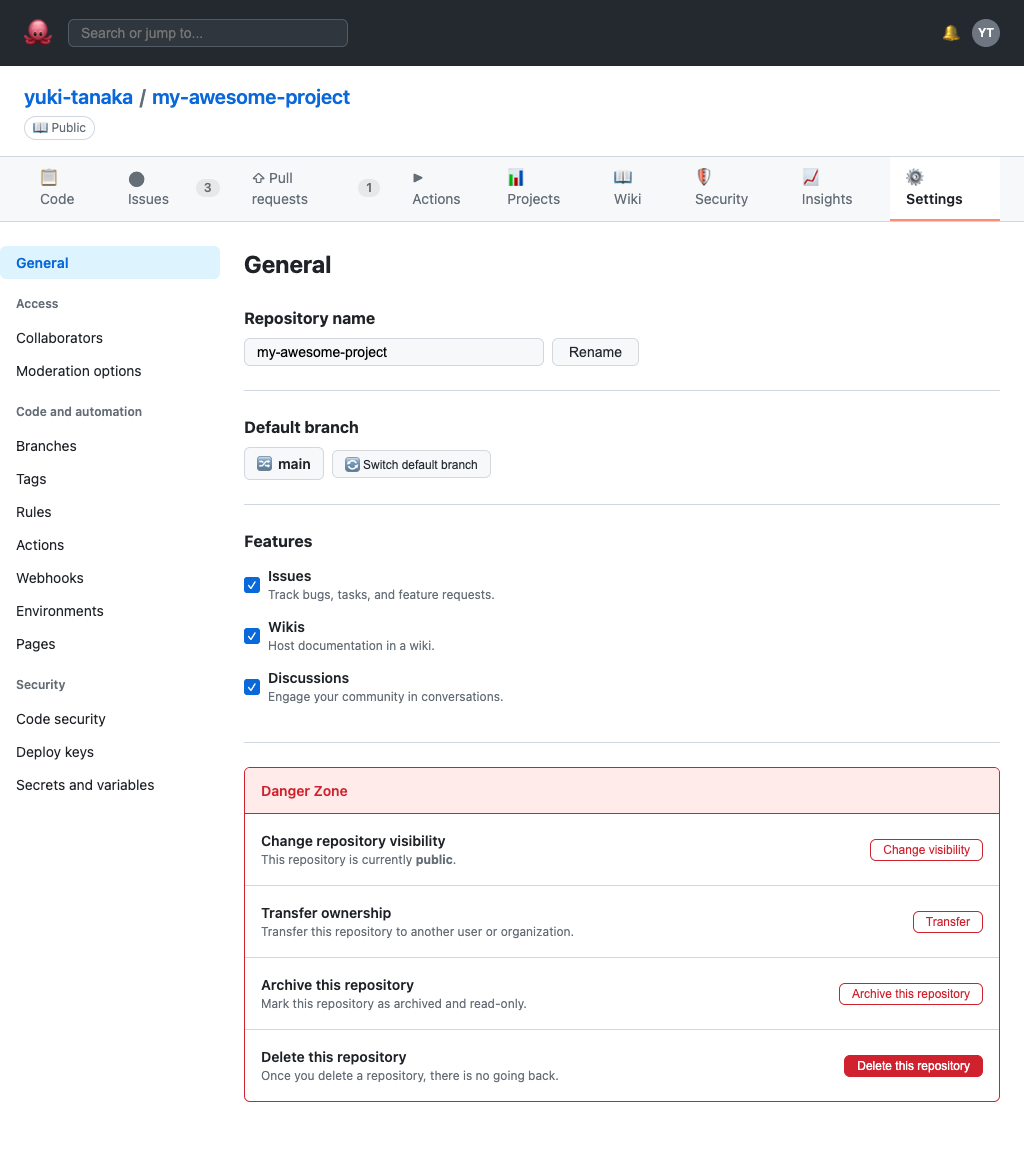
\includegraphics[width=0.95\textwidth]{images/repo-settings.png}
\caption{リポジトリのSettingsタブ画面}
\end{figure}

\subsubsection{リポジトリの可視性（Visibility）}

リポジトリの可視性は、誰がリポジトリの内容を閲覧できるかを制御します。

\begin{table}[htbp]
\centering
\begin{tabular}{llp{6cm}}
\hline
\textbf{設定} & \textbf{説明} & \textbf{適した用途} \\
\hline
\textbf{Public} & インターネット上の誰でも閲覧・クローン可能 & オープンソースプロジェクト、ポートフォリオ \\
\textbf{Private} & 招待された共同作業者のみアクセス可能 & 個人プロジェクト、企業の内部コード \\
\textbf{Internal} & Organization内のメンバーのみアクセス可能 & Enterprise向け、社内利用 \\
\hline
\end{tabular}
\end{table}

可視性はSettingsの「General」セクションで変更できます。また、GitHub CLIからも変更可能です。

\begin{lstlisting}[language=bash]
# リポジトリを公開に変更する
gh repo edit --visibility public

# リポジトリを非公開に変更する
gh repo edit --visibility private
\end{lstlisting}

PublicからPrivateへの変更は即座に反映されますが、既にForkされたリポジトリには影響しません。逆に、PrivateからPublicに変更する場合は、リポジトリの全履歴が公開されることに注意してください。

\subsubsection{ブランチ保護（Branch Protection Rules）}

チーム開発において非常に重要な機能が\textbf{ブランチ保護ルール}です。Settings の「Branches」セクションで設定できます。

ブランチ保護ルールを設定すると、たとえば \cmd{main} ブランチに直接プッシュすることを禁止し、必ずプルリクエストを経由してマージすることを強制できます。これにより、コードレビューを必ず通す運用が実現します。

主な保護設定には以下のものがあります。

\begin{itemize}
  \item \textbf{Require a pull request before merging}: マージ前にプルリクエストを必須にする
  \item \textbf{Require approvals}: 指定した人数のレビュー承認を必須にする
  \item \textbf{Require status checks to pass}: CI/CDのテストが成功しないとマージできなくする
  \item \textbf{Restrict who can push}: プッシュできるユーザーを制限する
\end{itemize}

\begin{figure}[htbp]
\centering
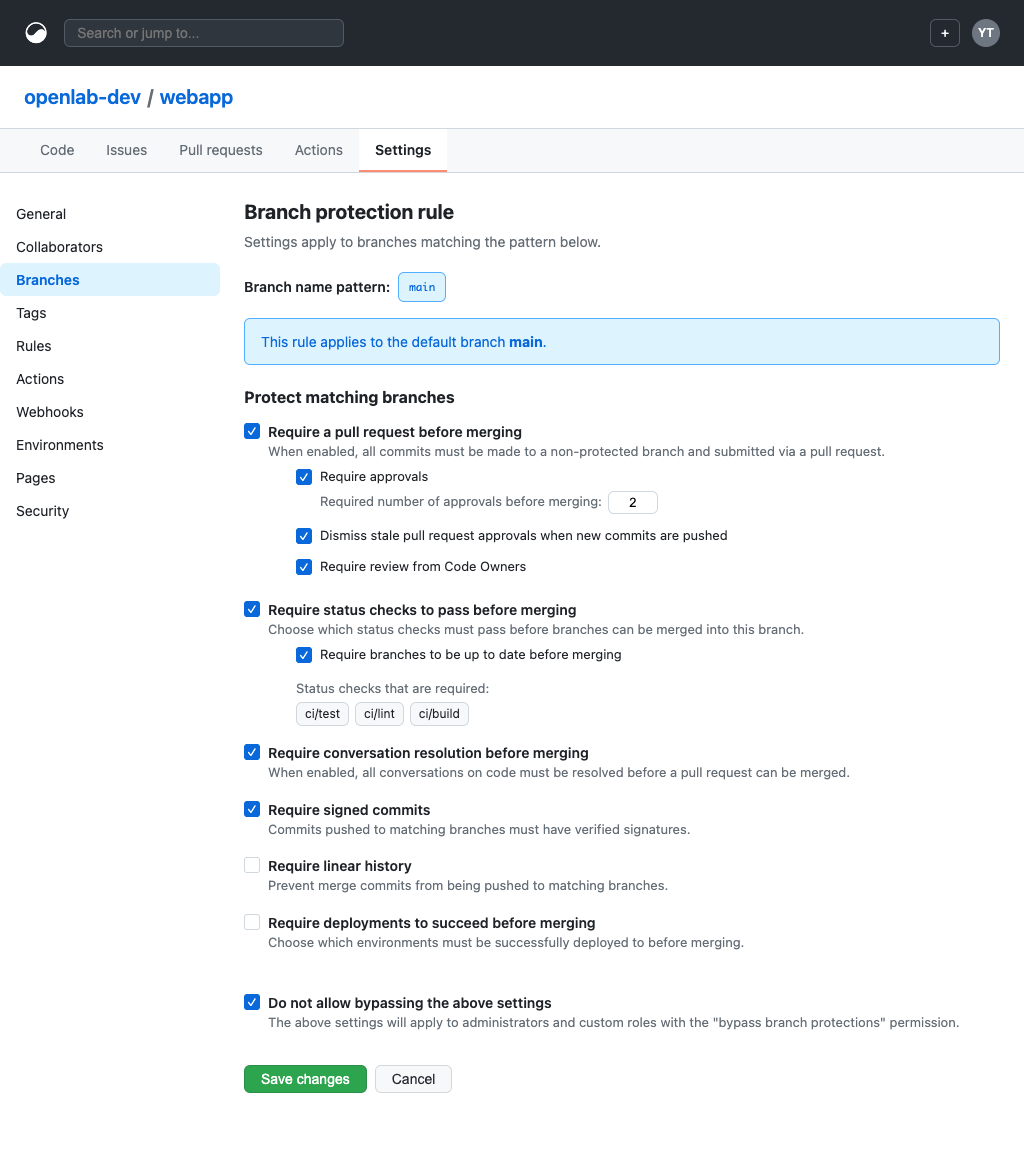
\includegraphics[width=0.95\textwidth]{images/branch-protection.png}
\caption{ブランチ保護ルールの設定画面}
\end{figure}

\subsubsection{Collaborators（共同作業者）}

Privateリポジトリで他の人と共同作業をする場合、Settings の「Collaborators」からユーザーを招待できます。招待されたユーザーは、リポジトリへのプッシュやプルリクエストの作成などが行えるようになります。

\subsection{テンプレートリポジトリ}

同じような構成のプロジェクトを何度も作成する場合、\textbf{テンプレートリポジトリ}を活用すると効率的です。テンプレートリポジトリから新しいリポジトリを作成すると、ファイル構造がコピーされますが、コミット履歴はコピーされません（新しい履歴がゼロから始まります）。

\textbf{テンプレートリポジトリの作成手順:}

\begin{enumerate}
  \item テンプレートにしたいリポジトリのSettingsを開く
  \item 「General」セクションの「\textbf{Template repository}」にチェックを入れる
\end{enumerate}

\textbf{テンプレートから新しいリポジトリを作成する手順:}

\begin{enumerate}
  \item テンプレートリポジトリのページで「\textbf{Use this template}」ボタンをクリック
  \item 「\textbf{Create a new repository}」を選択
  \item 通常のリポジトリ作成と同じように名前や設定を入力して作成
\end{enumerate}

\begin{lstlisting}[language=bash]
# GitHub CLIでテンプレートから作成する場合
gh repo create my-new-project --template username/template-repo --clone
\end{lstlisting}

テンプレートリポジトリは、チームの開発規約に沿ったプロジェクト構成（ディレクトリ構造、CI/CD設定、コーディングルールのファイルなど）を統一するのに非常に有効です。

\subsection{リポジトリの削除}

リポジトリを削除する場合は、Settings ページの最下部にある「\textbf{Delete this repository}」から実行できます。

\begin{lstlisting}[language=bash]
# GitHub CLIで削除する場合（確認プロンプトが表示される）
gh repo delete username/repo-name --yes
\end{lstlisting}

\begin{quote}
\textbf{注意}: リポジトリの削除は取り消せません。クローンを持っている人のローカルにはデータが残りますが、GitHub上からはイシュー、プルリクエスト、設定を含めてすべてが完全に削除されます。削除前に、本当に不要なリポジトリかどうかを確認してください。
\end{quote}

\section{まとめ}

この章では、Gitを使った作業の出発点であるリポジトリについて、その構造から作成・管理までを詳しく学びました。

\begin{itemize}
  \item \textbf{リポジトリの構造}: \cmd{.git} フォルダがリポジトリの心臓部であり、すべての変更履歴を保持している
  \item \textbf{作成方法}: GitHubで作成してクローンする方法が最も簡単で推奨される。ローカルで先に作業を始めた場合は \cmd{git init} してからGitHubに接続する
  \item \textbf{クローン}: \cmd{git clone} は単なるコピーではなく、リポジトリの完全な複製を作る。\cmd{--depth} や \cmd{--branch} などのオプションで動作をカスタマイズできる
  \item \textbf{リモート管理}: \cmd{origin} は自分のリモートリポジトリ、\cmd{upstream} はFork元を指す慣例的な名前
  \item \textbf{.gitignore}: ビルド成果物、依存パッケージ、機密情報、OS固有ファイルを除外する。既に追跡されたファイルは \cmd{git rm --cached} で解除が必要
  \item \textbf{リポジトリ設定}: 可視性の変更、ブランチ保護ルール、テンプレートリポジトリなど、GitHub上で多くの設定が可能
\end{itemize}

次の章では、リポジトリを作成した後の最も基本的な操作 — ファイルの変更を記録し、GitHubに共有するワークフローを学びます。
